\documentclass[12pt,AutoFakeBold]{article} 


\usepackage[科目名称]{BUAAreport}  
\problem{实验题目}  % 请在此处填写实验题目,最多支持两行题目(受封面大小限制),题目会自动换行
\tutor{XXX} % 同作者姓名
\labdate{\today} % 实验日期
%  如要采用学院、专业、学号、班级格式请在sty宏包更改,去掉注释即可
%  以下是学院,姓名,学号设置
\renewcommand{\studentid}{1234567890} % 用实际学号替换这里的数字
\renewcommand{\studentname}{张~大~三} % 实际姓名替换汉字
\renewcommand{\teachername}{李~小~四} % 实际指导老师姓名
\renewcommand{\overdate}{\today} % 默认完成时间为today,可手动修改,如:2024年11月28日
\renewcommand{\pagechead}{学号+姓名} % 页眉的学号和姓名

% !标题超过两行时,取消下面的三行注释,确保页眉仅有标题从而正常显示
%\chead{} 
%\rhead{}
%\fancyfoot[C]{\thepage}


% \usepackage{fourier}  % 这是 fourier 字体,更柔和 



%% 如果你需要中文的一级标题编号,如“一、”、“二、”等,请把下面两行取消注释
% \RequirePackage{zhnumber} % change section number to chinese
% \titleformat{\section}{\Large\bfseries\rmfamily}{\zhnum{section}、}{0em}{}

% 文档开始
        
\begin{document}

\maketitle
\setcounter{tocdepth}{2}
\tableofcontents  % 生成目录


% 正文标题
\makeatletter
\begin{center}
    \LARGE \textbf{\textsf{\@problem}}
\end{center}
\makeatother

% 正文开始

\section{选题目的}
当代人类社会已经进入到高度发达的信息化社会。信息化社会的发展离不开电子信息技术产品的开发、产品品质的提高和改善。EDA技术的发展和推广应用又极大地推动了电子信息产业的发展。为保证电子系统设计的速度和质量,适应“第一时间推出产品”的设计要求,EDA技术正逐渐成为不可缺少的一项先进技术和重要工具。

\begin{enumerate}
    \item 研究多功能数字钟的工作原理,进行功能设计;
    \item 加深VHDL语言的理解;
    \item 熟练掌握自上而下的分层设计方法;
    \item 熟练掌握EDA软件Quartus II的开发流程。
\end{enumerate}


\section{设计目标}
在实时钟电路设计的基础上增加以下功能。

\begin{itemize}
    \item \textit{正常}模式,增加上,下午显示。
    \item \textit{手动校准}电路。按动方式键,将电路置于校时状态,则计时电路可用手动方式校准,每按一下校时键,时计数器加1;按动方式键,将电路置于校分状态,以同样方式手动校分。
    \item \textit{整点报时},仿中央人民广播电台整点报时信号,从59分50秒起每隔2秒发出一次低音“嘟”信号(信号鸣叫持续时间1 s,间隙时间1 s)连续5次,到达整点(00分00秒时),发一次高音“哒”信号(信号持续时间1秒)。
    \item \textit{闹时}功能,按动方式键,使电路工作于预置状态,此时显示器与时钟脱开,而与预置计数器相连,利用前面手动校时,校分方式进行预置,预置后回到正常模式。当计时计至预置的时间时,扬声器发出闹铃信号,时间为半分钟,闹铃信号可以用开关“止闹”,按下此开关后,闹铃声立刻中止,正常情况下应将此开关释放,否则无闹时作用。
    \item \textit{秒表}功能。按START键开始计秒,按STOP键停止计秒并保持显示数不变,直到复位信号加入。 
\end{itemize}
 

\section{实现方案}
% 包括原理框图和VHDL设计程序
\subsection{仿真环境}
\begin{itemize}
    \item OS环境:Windows 10
    \item 处理器类型:x86\_64
    \item 软件名称:Quartus II
    \item Quartus II版本:9.0 Build 132 02/25/2009 SJ Full Edtion
    \item 器件库家族:Cyclone III
    \item 器件:EP3C16F484C6
\end{itemize}

\subsection{总体工作原理}
根据题目要求,我们可以将实现该数字钟的功能模块分为四类:\textit{输入层}(主要负责从引脚读入参数,并进行基本处理)、\textit{核心层}(主要负责时钟模块正常运行)、\textit{功能层}(主要负责实现整点报时、闹钟、秒表、上下午显示等功能模块)、\textit{输出层}(负责将时间或者设置显示到7段数码管)。如图 \ref{fig:map} 所示可以看出各层级包含的模块。
\begin{figure}[htbp]
    \centering
    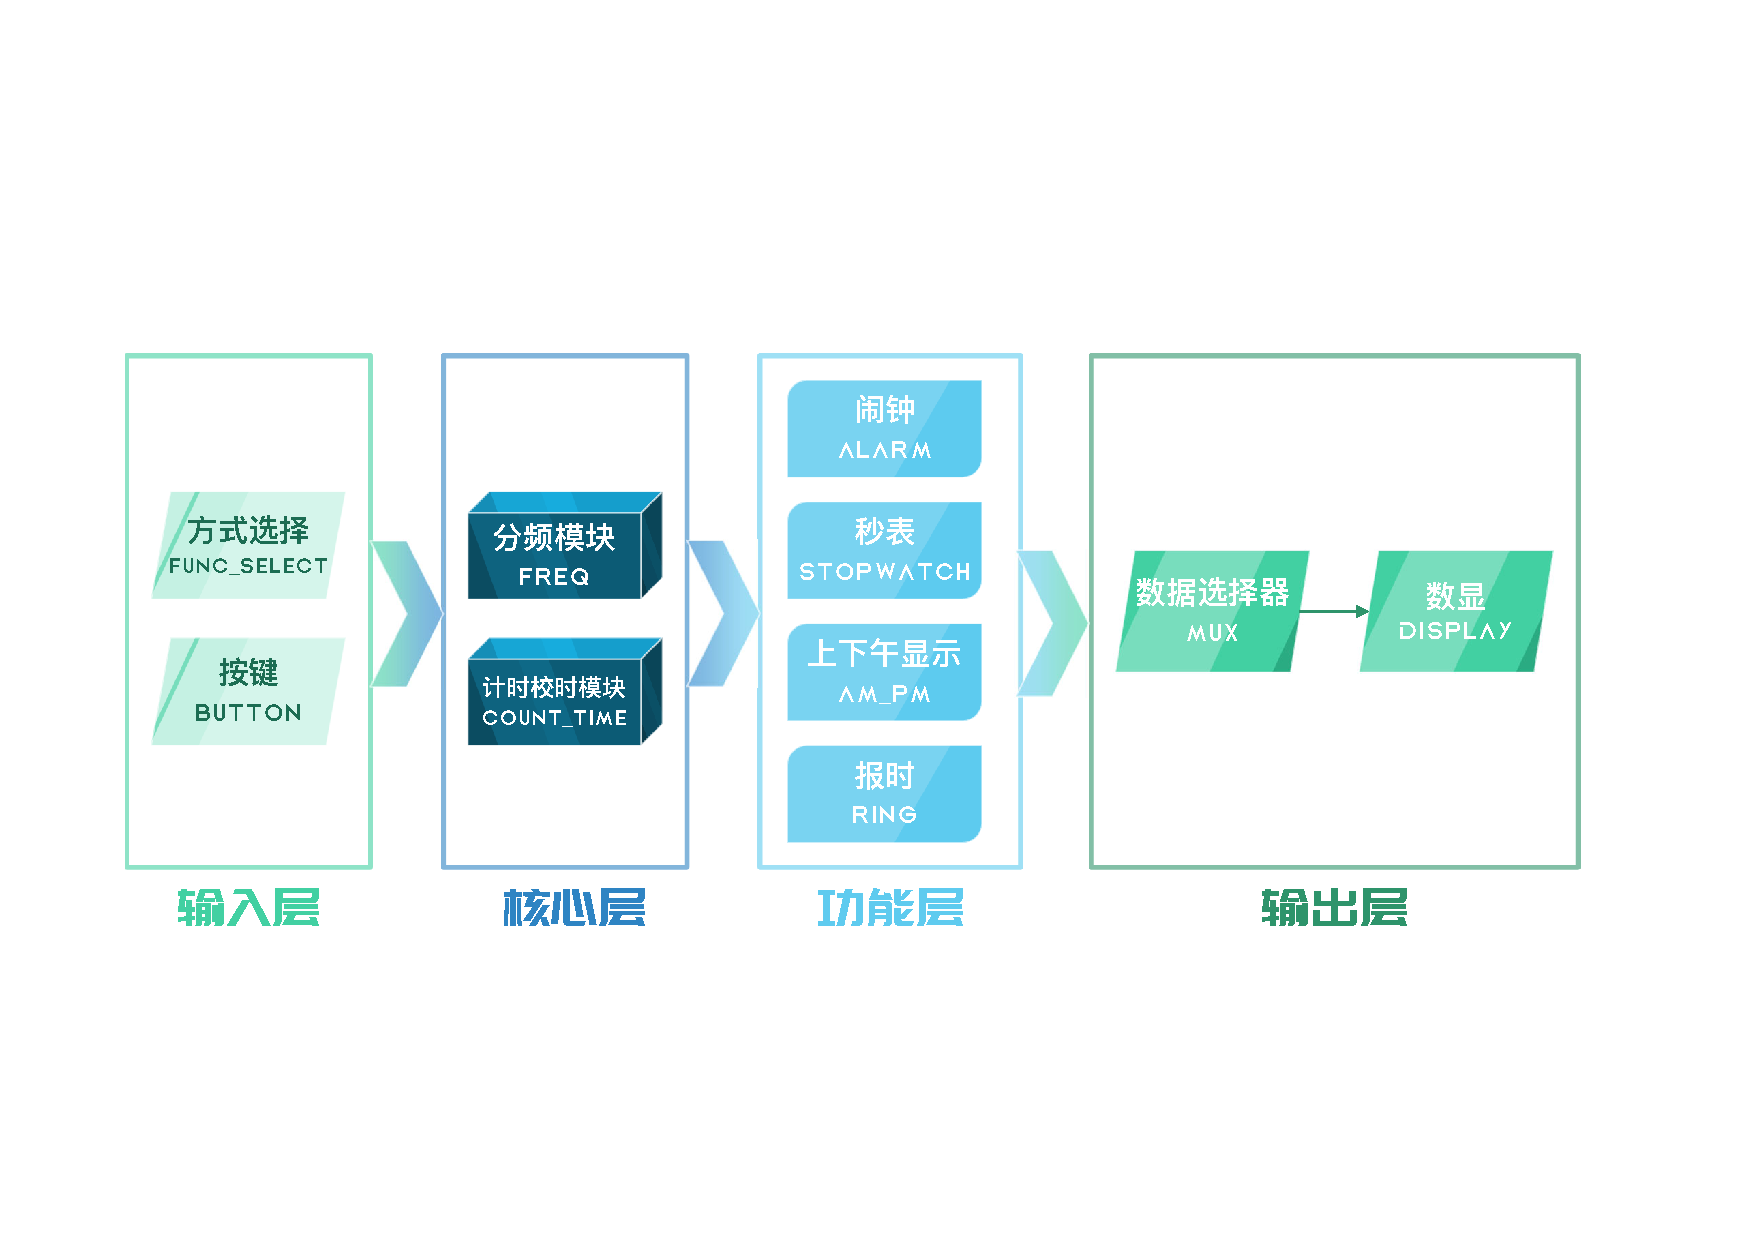
\includegraphics[width=.9\textwidth]{map.pdf} 	% 图片相对位置
    \caption{总体工作原理层级图}		% 图片标题 
    \label{fig:map}							% 图片标签
\end{figure}

利用\textit{自顶向下的层次化设计方式},用系统级行为描述表达一个包含输入输出的顶层模块,同时完成整个系统的模拟与性能分析。将系统划分为各个功能模块,每个模块由更细化的行为描述表达。
于是,我们可以将上述层次图转化为Quartus中的BDF原理图,设置每个模块的I/O端口,如图 \ref{fig:Smart_Clock_bdf} 所示可以看出各层级、各模块间的映射关系。
\begin{landscape}

\begin{figure}[htbp]
    \centering
    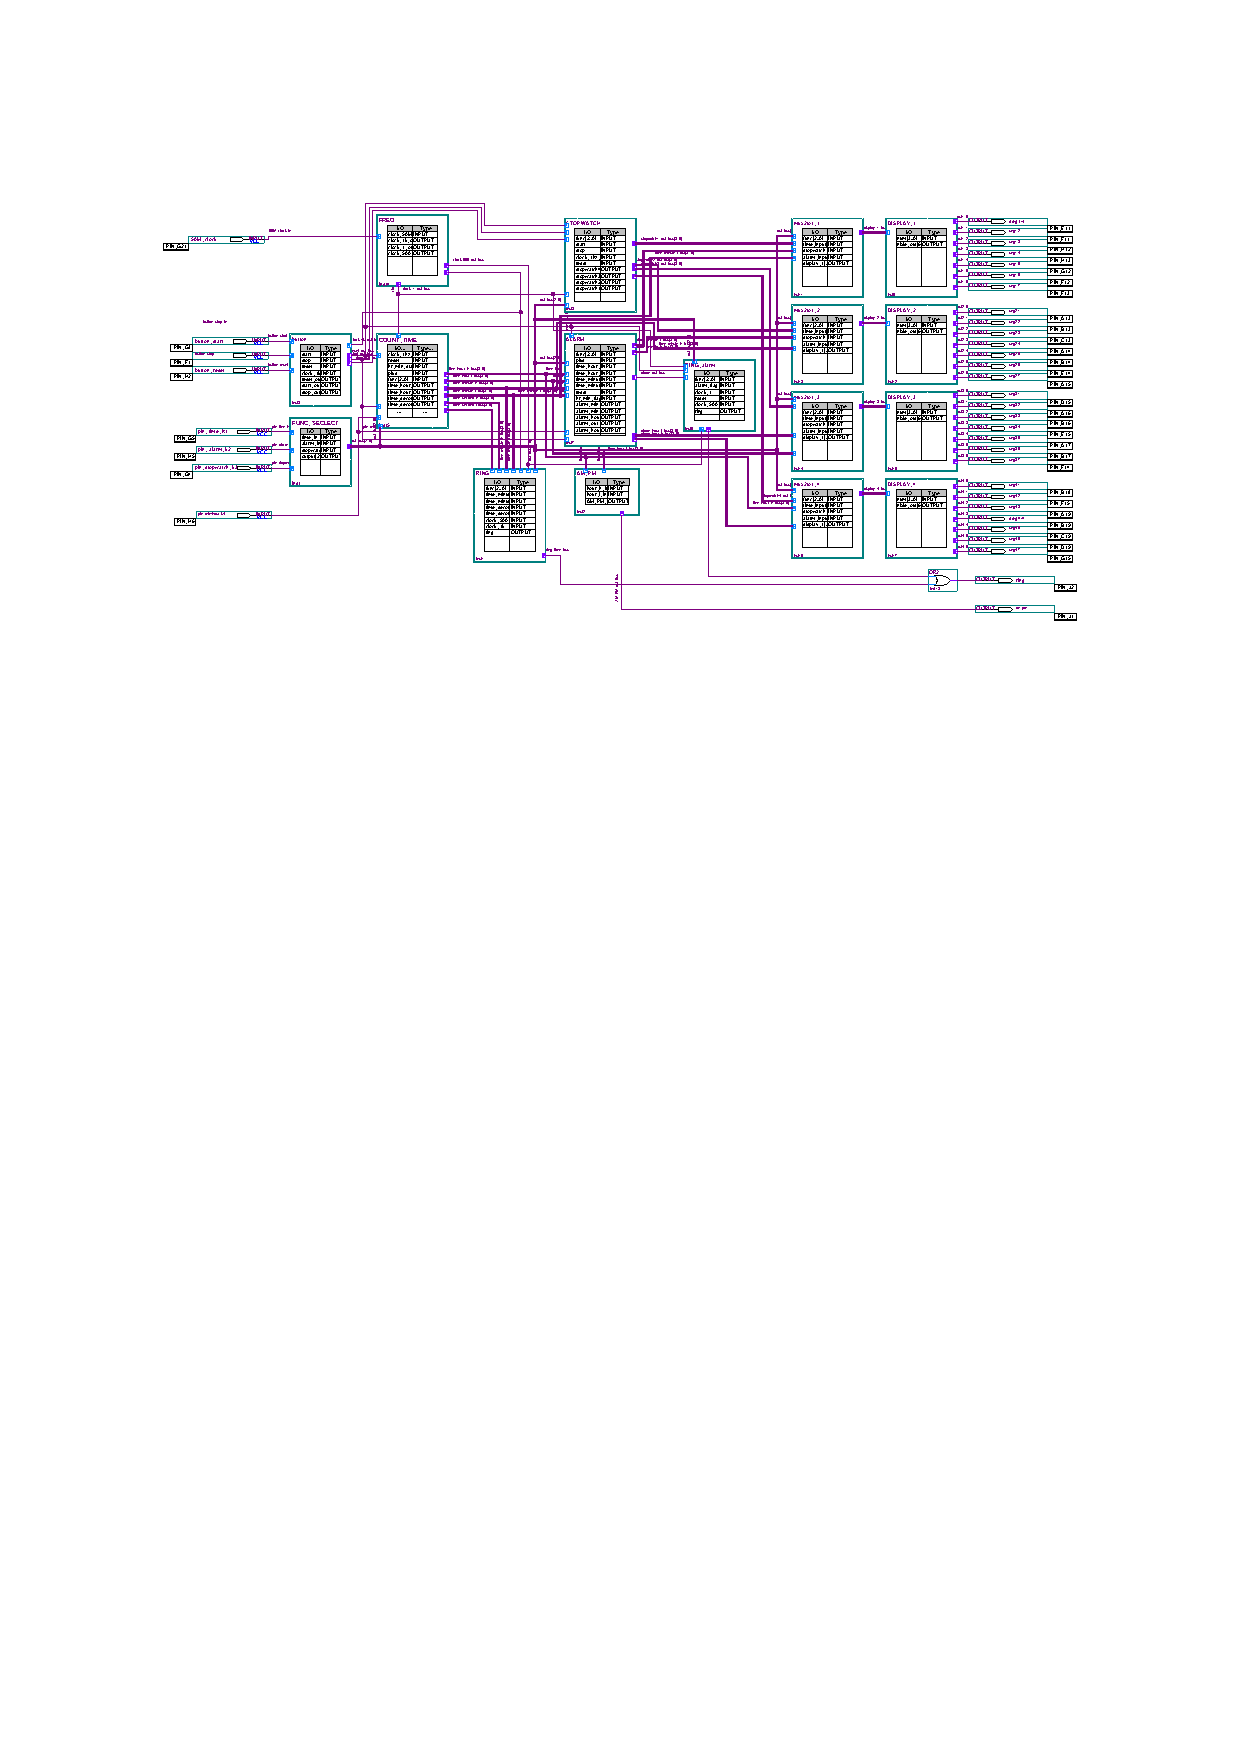
\includegraphics[width=1.65\textwidth]{Smart_Clock_bdf.pdf} 	% 图片相对位置
    \caption{多功能数字钟的BDF原理图}		% 图片标题 
    \label{fig:Smart_Clock_bdf}							% 图片标签
\end{figure}
\end{landscape}

从图 \ref{fig:Smart_Clock_bdf} 中可以看出,该数字钟有8个外部输入:时钟\textsf{50M\_clock}
\footnote{在本文中,我们用等宽字体表示模块(如\texttt{FREQ}) 或者代码函数等(如\texttt{case});用无衬线字体表示信号、变量等(如\textsf{time\_hour\_l});用斜体表示外部输入异步信号(如\textit{RESET});用加粗字体代表向量(如1001111);用加粗的无衬线体表示当前状态(如\textsf{\textbf{校时}}、\textsf{\textbf{秒表}})。}
、4个逻辑开关($K_1$校时、$K_2$闹钟、$K_3$秒表、$K_4$时/分选择)、3个按键(\textit{START/PLUS}、\textit{STOP}、\textit{RESET})。有30个外部输出:4个7段数码管输出、1个音频输出、1个上下午指示。\footnote{外部输入输出的映射见第 \ref{sec:result} 节 \textbf{实现结果}。}

\subsection{分模块原理框图}
从图 \ref{fig:Smart_Clock_bdf} 中我们已经能大致看出该系统的工作方案\footnote{下述各\textit{Step}间为顺序运行的关系,而\textit{Step}内的小点为并行运行的。}为:

XXX


\section{设计过程与仿真结果}
下面对较为关键模块的实现过程进行详细的叙述,主要包括按键(\texttt{BUTTON})模块、分频(\texttt{FREQ})模块、计时校时(\texttt{COUNT\_TIME})模块、闹钟(\texttt{ALARM}、\texttt{RING\_ALARM})模块、秒表(\texttt{STOPWATCH})模块、报时(\texttt{RING})模块。而对于方式选择(\texttt{FUNC\_SELECT})模块、上下午显示(\texttt{AM\_PM})模块、数据选择器(\texttt{MUX})模块、数显(\texttt{DISPLAY})模块则在第 \ref{subsec:others} 小节一带而过。具体的VHDL代码详见附录。


\subsection{\texttt{COUNT\_TIME}模块实现过程}
\subsubsection{\texttt{COUNT\_TIME}模块设计流程}
计时校时(\texttt{COUNT\_TIME})模块其实是一个非常重要的模块,它对于闹钟、上下午显示、报时等功能都有着至关重要的影响,同时它也是闹钟最基本的功能。我原计划将这部分分为计时(\texttt{COUNT\_TIME})、校时(\texttt{PROOFREAD})两个模块,但是由于设计上出了一点问题\footnote{我想在两个进程中改变同一个信号,但是这并不可行,但是其实可以将两个信号再或起来,就能实现这个功能。我最后也是这么实现的。},所以不得不将两部分合为一块。

计时校时的基本思路如流程图 \ref{fig:map_count_time} 所示。在这个模块中有4个并行的进程:校时进程、秒进程、分进程、时进程。
\begin{figure}[htbp]
    \centering
    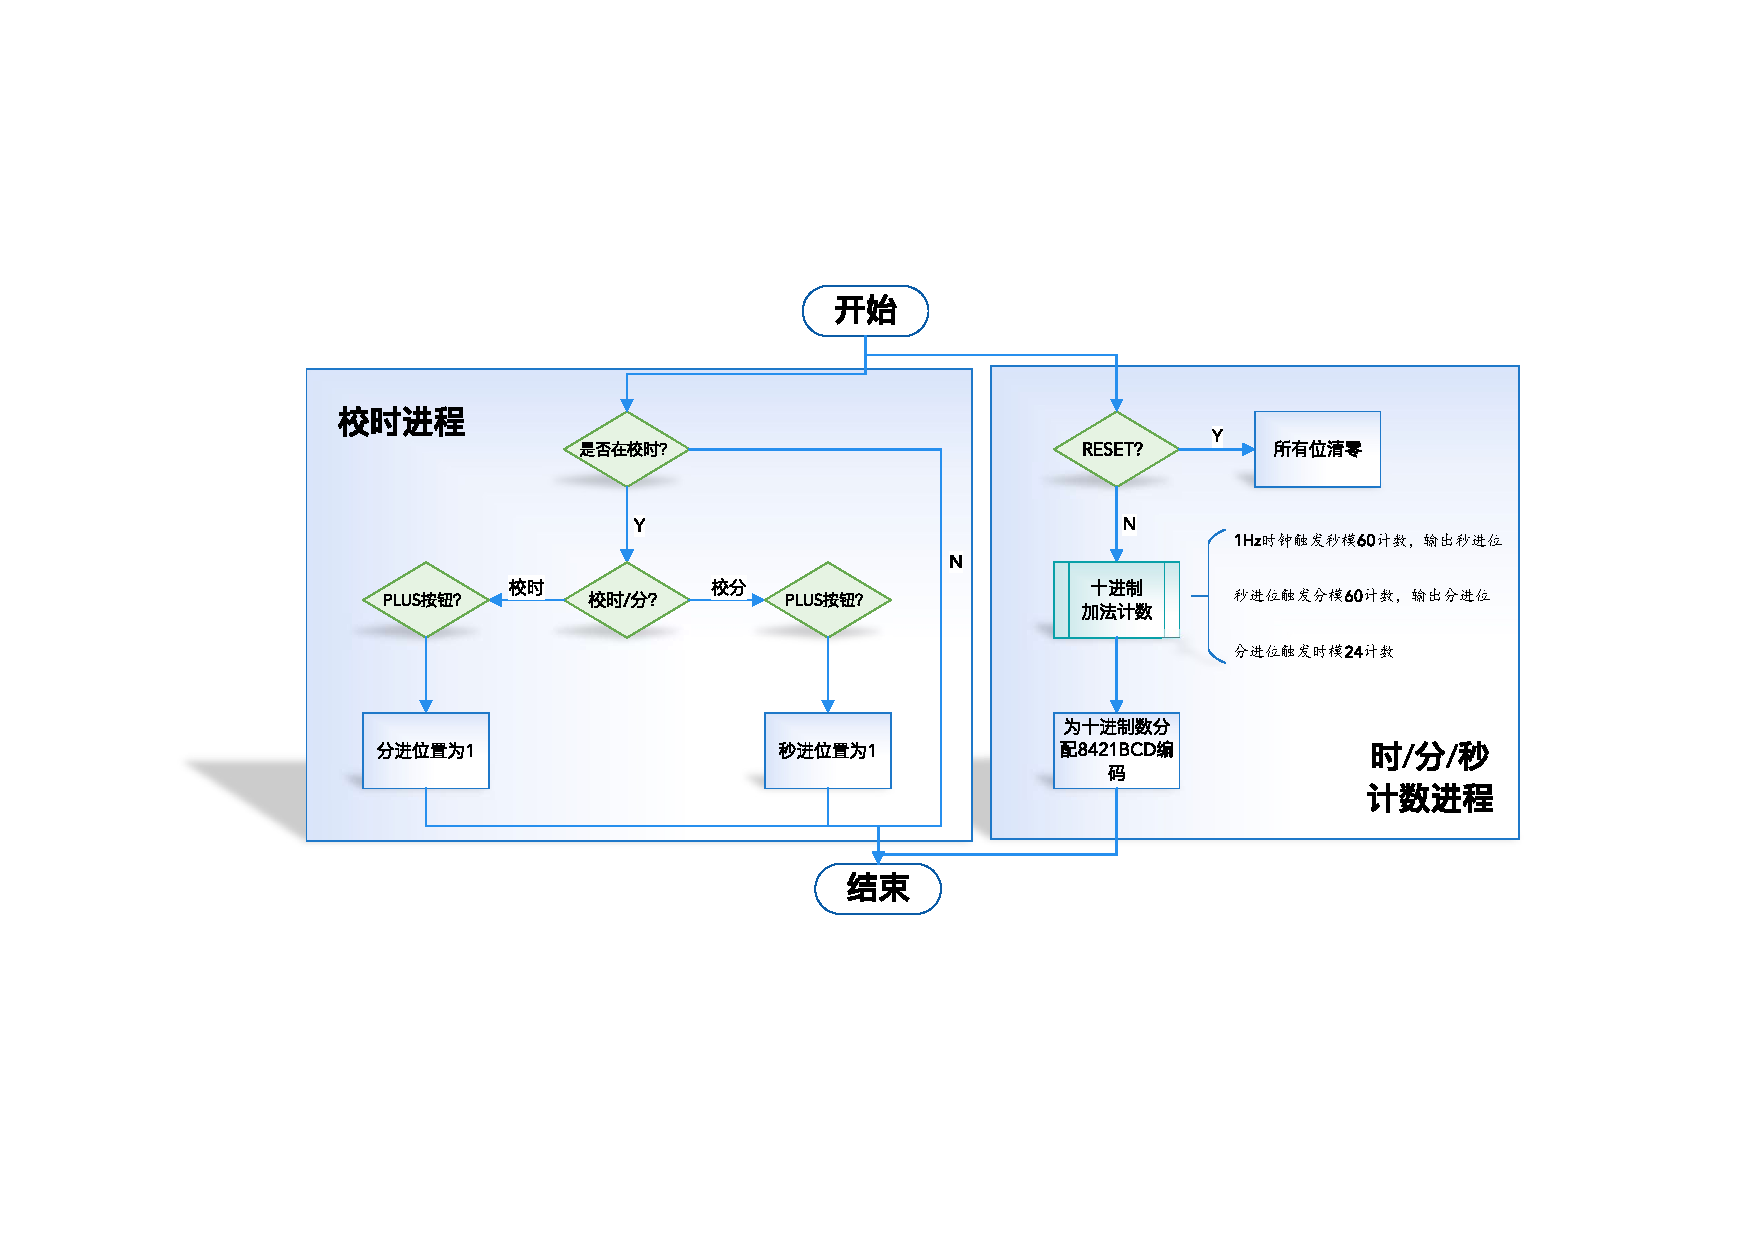
\includegraphics[width=.9\textwidth]{map_count_time.pdf} 	% 图片相对位置
    \caption{计时校时流程框图}		% 图片标题 
    \label{fig:map_count_time}							% 图片标签
\end{figure}

这个模块最重要的就是处理好外部\textit{校时异步信号}\textsf{plus}和内部\textit{进位信号}\textsf{couts、coutm}之间的关系。我一开始的想法是,这两个信号是一体的,外部信号和进位信号改变的是同一个信号,但这并不可行,会报错\textit{“不能两个进程同时改变一个信号”}。最后的处理办法是将校时产生的进位信号和内部计时产生的进位信号分开处理,最后在并行处理的部分将两个信号或起来即可实现比较好的效果。下面以分计数(秒对分的进位)为例,予以说明。

我们首先在结构体中声明以下几个信号:
\begin{lstlisting}[language=vhdl,numbers=none]
    signal couts:STD_LOGIC;     --分计时触发信号
    signal couts1:STD_LOGIC;    --校分产生的进位加信号
    signal couts2:STD_LOGIC;    --秒计数至60产生的进位信号
    \end{lstlisting}
    
在校时进程中,我们有这样的分支程序(这只是校分的部分):
\begin{lstlisting}[language=vhdl,numbers=none]
if(hr_min_state='0') then 	--校分
    if(plus='1') then 
        couts1<='1';
    else
        couts1<='0';
    end if;
end if;
    \end{lstlisting}
秒计数进程为:
\begin{lstlisting}[language=python]
second: process(clock_1hz_in,reset)  --进程second开始
variable temp1s:integer range 0 to 10;
variable temp2s:integer range 0 to 6;
begin
    if (reset='1') then
        temp1s:=0;
        temp2s:=0;
    elsif (clock_1hz_in'event and clock_1hz_in='1') then
        temp1s:=temp1s+1;
        if (temp1s=10) then
            temp1s:=0;
            temp2s:=temp2s+1;
            if (temp2s=6) then
                temp2s:=0;
                couts2<='1';
            else
                couts2<='0';
            end if;
        end if;
    end if;
    case temp1s is
        when 0=>time_second_l<="0000";
        when 1=>time_second_l<="0001";
        when 2=>time_second_l<="0010";
        when 3=>time_second_l<="0011";
        when 4=>time_second_l<="0100";
        when 5=>time_second_l<="0101";
        when 6=>time_second_l<="0110";
        when 7=>time_second_l<="0111";
        when 8=>time_second_l<="1000";
        when 9=>time_second_l<="1001";
        when others=>null;
    end case;
    case temp2s is
        when 0=>time_second_h<="0000";
        when 1=>time_second_h<="0001";
        when 2=>time_second_h<="0010";
        when 3=>time_second_h<="0011";
        when 4=>time_second_h<="0100";
        when 5=>time_second_h<="0101";
        when others=>null;
    end case;
end process;
\end{lstlisting}

\begin{lstlisting}[language=python]
print("hello,BUAA")
\end{lstlisting}

这样我们在校时进程和秒计数进程中分别改变信号\textsf{couts1、couts2}的值,互不影响,不会报错。接着,我们在结构体中增加一个“或”语句,将上述改变的两个进位信号合并为一个信号\textsf{couts},并以此作为敏感信号来触发分计数。\footnote{其实这样的做法也不是很好,因为一般不能把组合逻辑的输出作为后续的敏感信号,这会导致竞争和冒险,产生毛刺。}
\begin{lstlisting}[language=vhdl,numbers=none]
    couts<=couts1 or couts2;

    minute: process(couts,reset) --进程minute开始
    \end{lstlisting}

同样地,在校时进程和分计数进程中分别改变信号\textsf{coutm1、coutm2}的值,将其相“或”获得分进位信号\textsf{coutm},并以此作为敏感信号来触发时计数。其完整的VHDL程序见附录\ref{subsec:B}。

这部分最后输出的就是多功能数字钟的本体——最基础的时/分/秒时钟信号。

\subsubsection{\texttt{COUNT\_TIME}模块仿真结果}
将\texttt{COUNT\_TIME}模块设为顶层实体,并建立\texttt{COUNT\_TIME}模块对应的vwf波形文件,导入相应的节点。
我们对\texttt{COUNT\_TIME}可能会出现的各种情况进行了仿真,得到的波形图如图 \ref{fig:count_time_wave} 所示。
\begin{figure}[htbp]
    \centering
    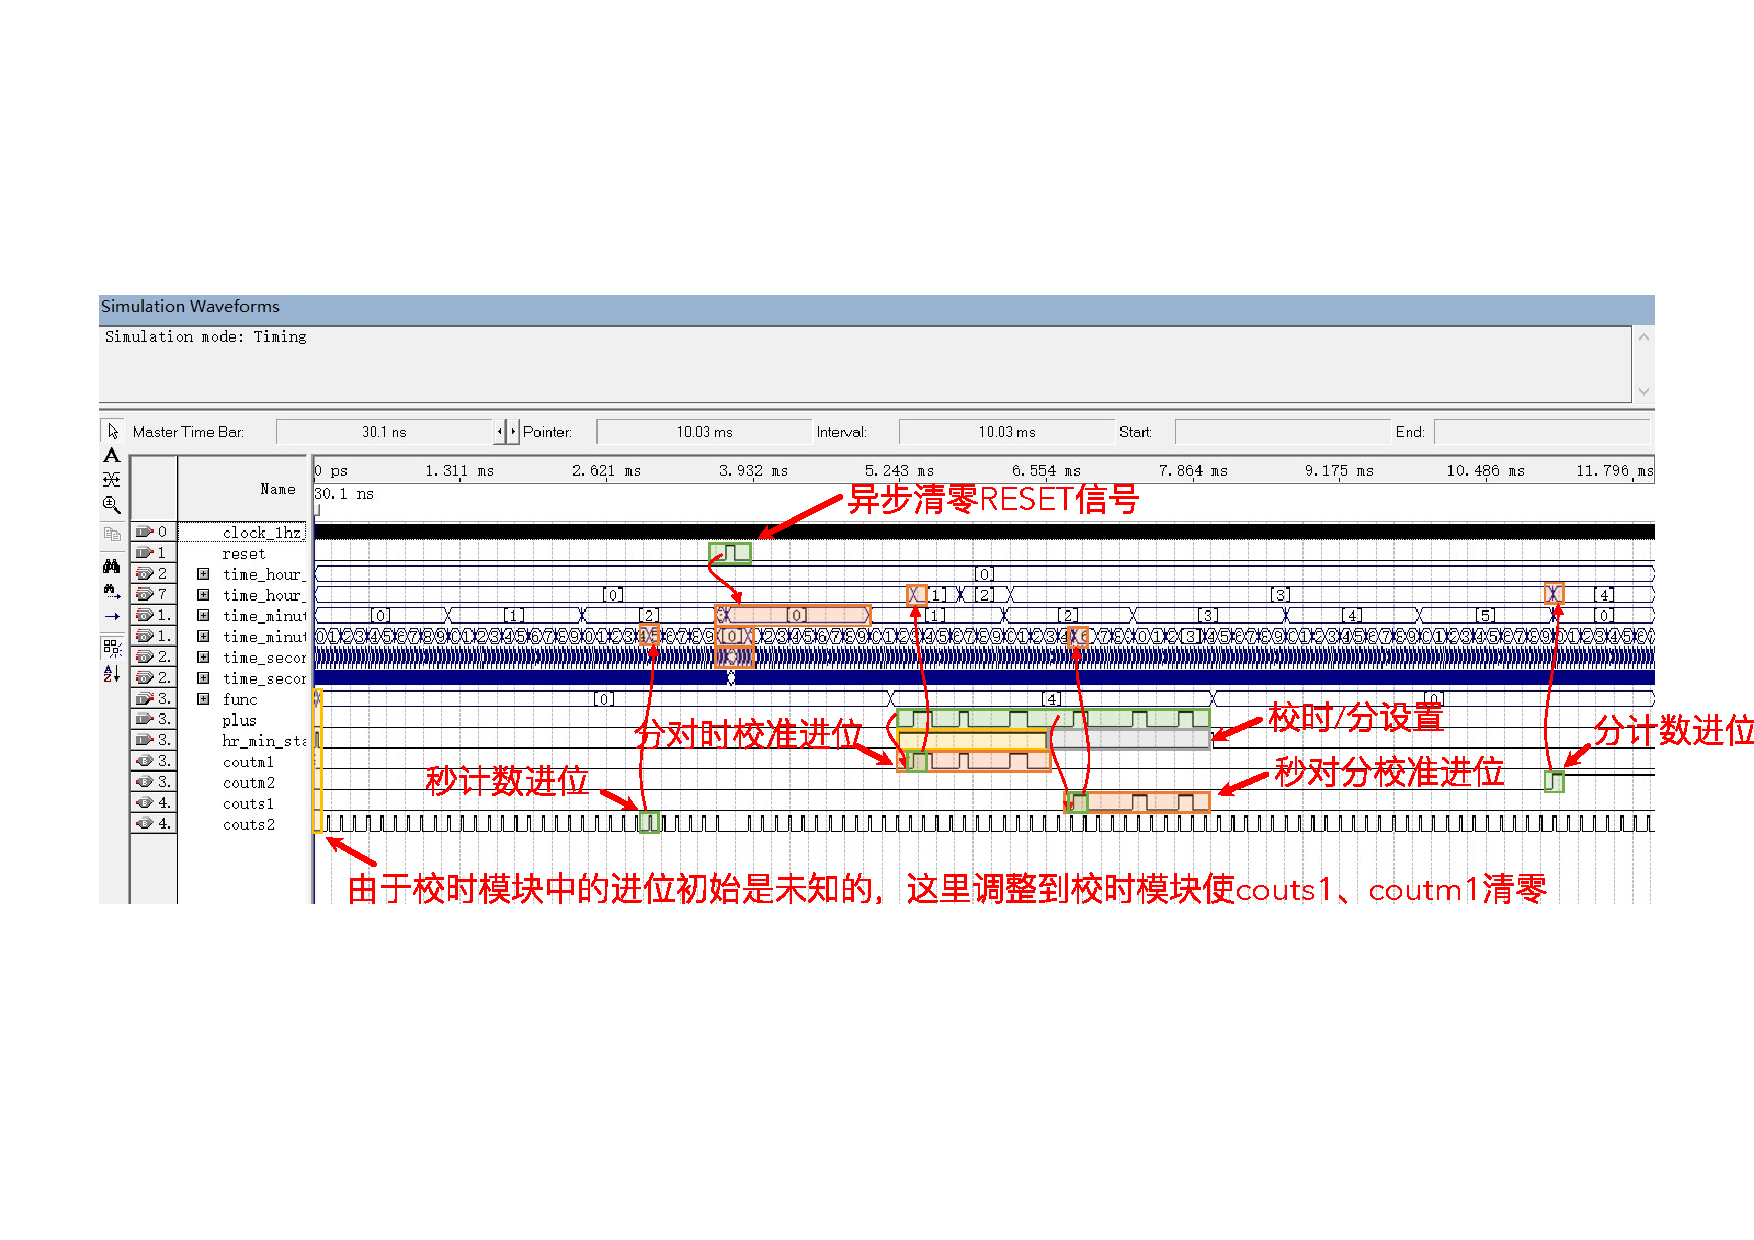
\includegraphics[width=\textwidth]{count_time_wave.pdf} 	% 图片相对位置
    \caption{\texttt{COUNT\_TIME}模块仿真结果}		% 图片标题 
    \label{fig:count_time_wave}							% 图片标签
\end{figure}

如图 \ref{fig:count_time_wave},这里我们只是为了说明进位和校时的规则,所以并没有将时钟设置为1 Hz。由于在仿真中各波形的状态是未定的,所以在仿真波形最开始,我们先将方式设置为\textsf{\textbf{校时}}模式,将校时秒进位\textsf{couts1}、校时分进位\textsf{coutm1}清零。在正常的\textsf{\textbf{时钟}}模式下,我们可以看到秒进位和分进位可以很好的触发分和时的计数,异步的清零\textsf{reset}信号也可以将所有的时间清零。在\textsf{\textbf{校时}}模式下,外部输入的校时异步信号\textsf{plus}可以在校时/分设置的指示下,正确的调整时钟的时间。

\subsection{其余模块实现过程}\label{subsec:others}
针对剩余模块,这里只给出设计思路,不再对其进行仿真。


\subsubsection{\texttt{DISPLAY}模块实现过程}
由于在DE0板上使用的是共阳极数码管,这里查表 \ref{tb:display} 可以得到显示字符和共阳极段码的对应关系,同时我们不需要小数点指示灯亮,所以最高位这里默认接‘\textbf{0}’。

这里使用\texttt{case}语句来实现显示数值和共阳极二进制段码的转换。


\section{遇到问题及解决方法}
\begin{enumerate}[\sffamily 1.]
    \item {\kaishu 进行编译时无法只编译对应的模块。进行波形图仿真无法引入正确的节点,同时无法生成我所需要的节点的波形。}
    
    {\heiti 解决方法:}通过查询网络上的资料,发现在Quartus II 9.0版本进行单模块编译和波形仿真的操作有以下几步:
    \begin{enumerate}[S1:]
        \item 将对应的模块设为顶层实体,进行编译;
        \item 将当前仿真文件设置为对应的波形文件(\textsf{Assignments}$\to$\textsf{Settings}$\to$\textsf{Simulator Settings})。
        \item 点击“\textsf{Start Simulation}”,开始波形仿真。
    \end{enumerate}
    \item {\kaishu 在校时和调整闹钟时,传来闹钟铃响和整点报时的铃声。}
    
    {\heiti 解决方法:}闹钟铃响和整点报时都有一个大前提,那就是当前数字钟处在\textsf{\textbf{时钟(报时)}}功能。这样就能够避免校时和调整闹钟时传来闹钟铃响和整点报时的铃声。
\end{enumerate}


\section{实现结果}\label{sec:result}
\subsection{DE0实验板的管脚分配}
对DE0实验板进行管脚分配,对应的一些按钮和按键的管脚\footnote{由于板子上没有扬声器,所以用LED灯来指示。}如表 \ref{tb:pin},对应位置如图 \ref{fig:DE0}。

\begin{table}[!htb]
    \begin{center}
    \caption{管脚分配}
    \begin{tabular}{lcc}
        \toprule
        名称    &实验板名称&GPIO管脚序号\\
        \midrule
        $K_1$校时开关   &SW[4]& G5\\ 
        $K_2$闹钟开关   &SW[1]& H5\\ 
        $K_3$秒表开关   &SW[3]& G4\\ 
        $K_4$时/分开关   &SW[2]& H6\\ 
        $START/PLUS$   &BUTTON[1]& G3\\ 
        $STOP$   &BUTTON[2] & F1\\ 
        $RESET$   &BUTTON[0] & H2\\ 
        上下午指示灯   &LEDG[0]& J1\\ 
        铃声   &LEDG[1]& J2\\ 
        \bottomrule
    \end{tabular}\label{tb:pin}
    \end{center}
\end{table}

\begin{figure}[htbp]
    \centering
    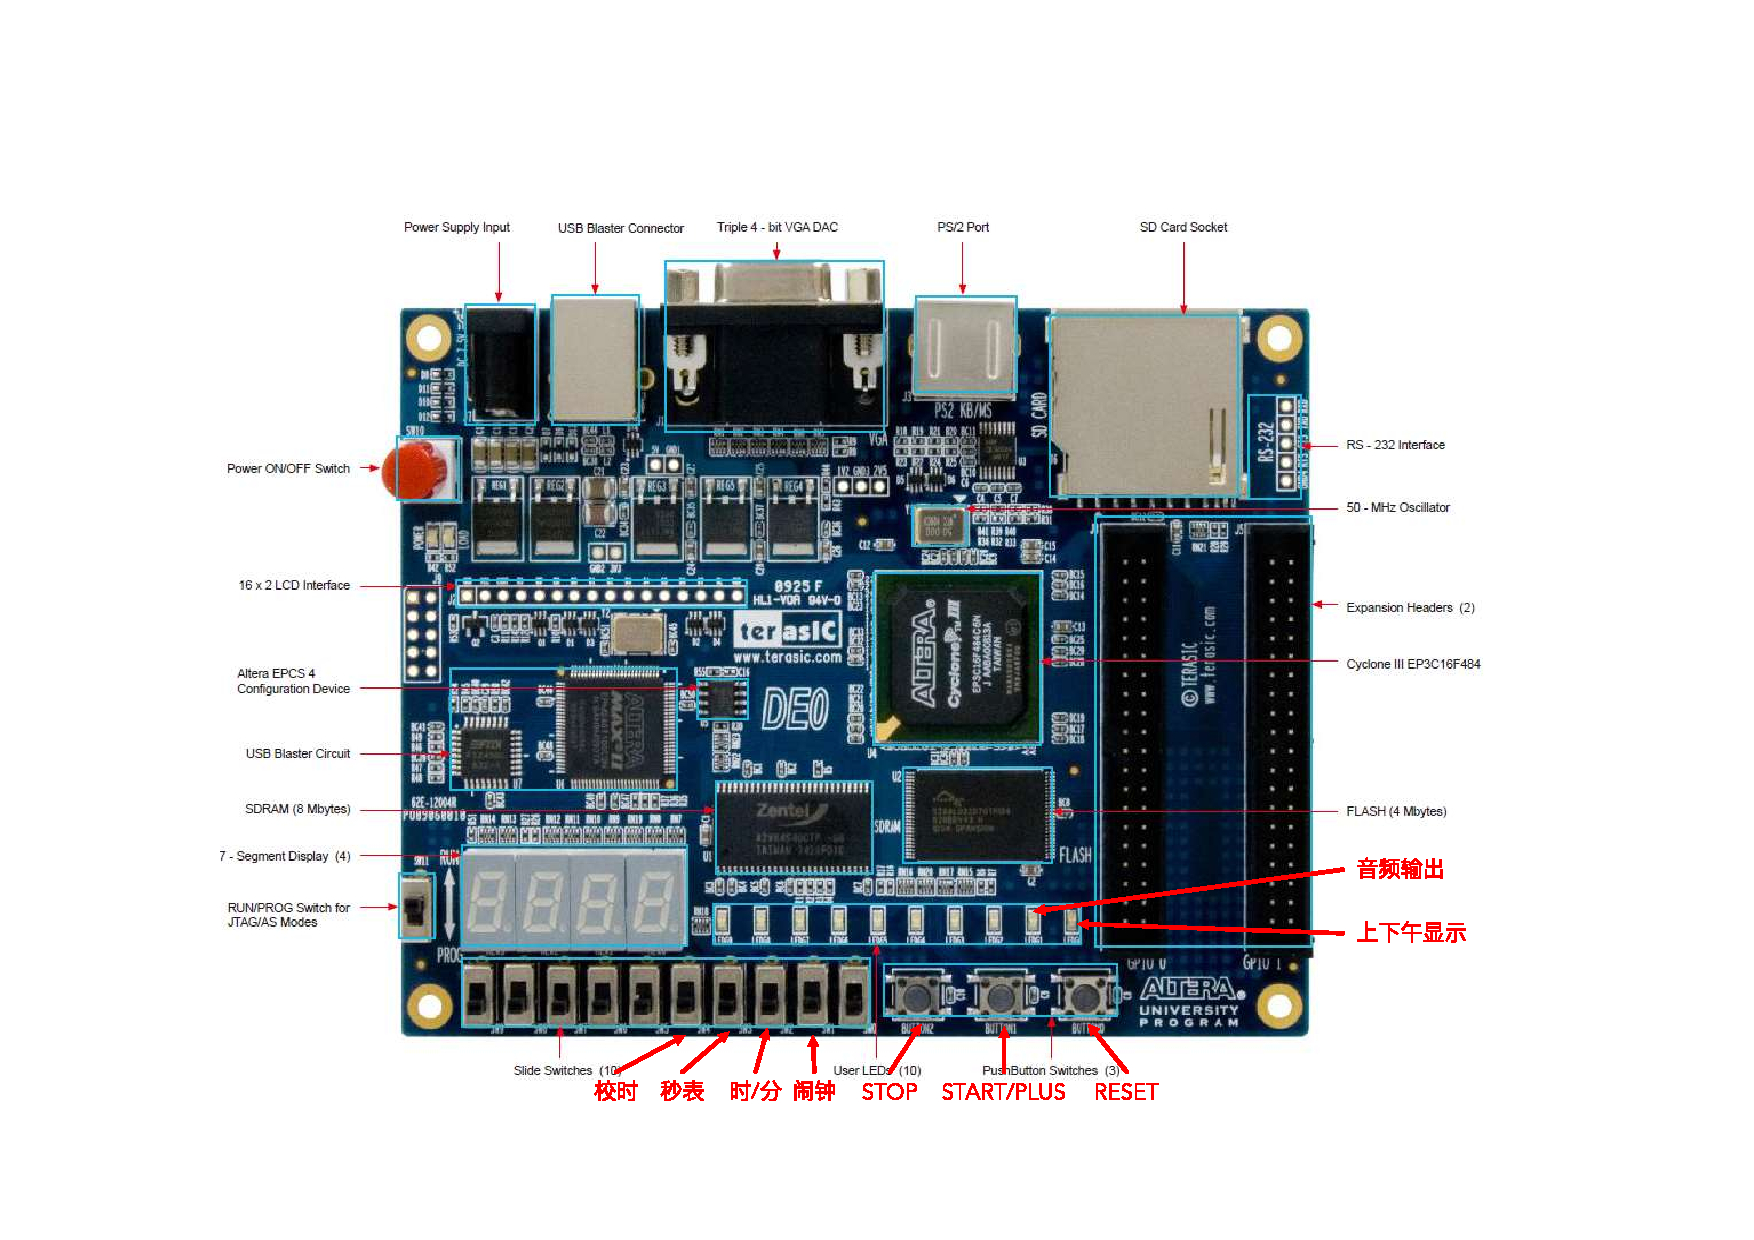
\includegraphics[width=.8\textwidth]{DE0.pdf} 	% 图片相对位置
    \caption{DE0实验板上对应的位置}		% 图片标题 
    \label{fig:DE0}							% 图片标签
\end{figure}

\subsection{上板调试}


\subsection{实现功能说明}
由于整体仿真难度比较大,本文不再对整个系统进行整体仿真。这边直接给出当前系统在实验板上能够完成并成功复现的所有功能。


% \section{编程调试(可选)}

\section{对该课程的实施意见及建议}
\begin{enumerate}
    \item XXXXXXXXXXXXXXXXXXXXXXXXX
    \item XXXXXXXXXXXXXXXXXXXXXXXXX
\end{enumerate}

% % 参考文献,此处以 MLA 引用格式为例

 \begin{thebibliography}{9}
    \bibitem{xiaodou} 言丶武.用VHDL编写简单的按键消抖程序[EB/OL].\url{https://www.jianshu.com/p/565896d5dcbb},2017-05-13/2020-09-27.
    %  \bibitem{2} 杨建国.新概念模拟电路(电子版全集)[M/OL].\url{https://www.analog.com/cn/landing-pages/002/yang-e-book.html},2018.

%     \bibitem{2} Clemente, Filipe Manuel, et al. "General network analysis of national soccer teams in FIFA World Cup 2014." \emph{International Journal of Performance Analysis in Sport} 15.1 (2015): 80-96.
%     \bibitem{3} Dijkstra, Edsger Wybe. "A Note on Two Problems in Connexion With Graphs." \emph{Numerische Mathematik} 1(1959):269-271.
 \end{thebibliography}
% % \includepdf[pages={1,2}]{Memo.pdf} 
% 可以直接导入pdf页面
\newpage
\begin{appendices}  % 附录环境

% \section{附录}
\section{核心层}\label{subsec:B}
% \noindent \textsc{\texttt{FREQ} Module} - \textbf{FREQ.vhd}
% \lstinputlisting[language=vhdl]{./code/FREQ.vhd}
此处是附录XXXX
       
    \end{appendices}
\end{document}  % 结束